\documentclass{article}
\usepackage[utf8]{inputenc}
\usepackage{graphicx}
\usepackage{amsthm}
\usepackage{amsmath}
\usepackage{amssymb}
\usepackage{float}
\usepackage{hyperref}
\usepackage{booktabs}
\usepackage[linesnumbered,ruled,vlined]{algorithm2e}
\usepackage{caption}
\usepackage{blkarray}
\usepackage{todonotes}
\usepackage{mathtools}
\usepackage[backend=biber,style=authoryear,natbib=true,url=false]{biblatex}

\addbibresource{references.bib}



%%%%%%%%%%%%%%%%%%%%%%%%%%%%
% Paper dependent stuff    %
%%%%%%%%%%%%%%%%%%%%%%%%%%%%

\newcommand{\Tau}{\mathcal{T}}

%%%%%%%%%%%%%%%%%%%%%%%%%%%%
% Aesthetics               %
% over-underline, hat, bold%
%%%%%%%%%%%%%%%%%%%%%%%%%%%%

\newcommand{\eps}{\varepsilon}
\newcommand{\vareps}{\varepsilon}
\renewcommand{\epsilon}{\varepsilon}
%\renewcommand{\hat}{\widehat}
\renewcommand{\tilde}{\widetilde}
\renewcommand{\bar}{\overline}

\newcommand*{\MyDef}{\mathrm{\tiny def}}
\newcommand*{\eqdefU}{\ensuremath{\mathop{\overset{\MyDef}{=}}}}% Unscaled version
% \newcommand*{\eqdef}{\mathop{\overset{\MyDef}{\resizebox{\widthof{\eqdefU}}{\heightof{=}}{=}}}}
\newcommand{\eqdef}{\stackrel{def}{=}}


\def\:#1{\protect \ifmmode {\mathbf{#1}} \else {\textbf{#1}} \fi}
\newcommand{\CommaBin}{\mathbin{\raisebox{0.5ex}{,}}}

\newcommand{\wt}[1]{\widetilde{#1}}
\newcommand{\wh}[1]{\widehat{#1}}
\newcommand{\wo}[1]{\overline{#1}}
\newcommand{\wb}[1]{\overline{#1}}

% bf and bm missing due to conflict!!
\newcommand{\bsym}[1]{\mathbf{#1}}
\newcommand{\bzero}{\mathbf{0}}
\newcommand{\ba}{\mathbf{a}}
\newcommand{\bb}{\mathbf{b}}
\newcommand{\bc}{\mathbf{c}}
\newcommand{\bd}{\mathbf{d}}
\newcommand{\be}{\mathbf{e}}
\newcommand{\bg}{\mathbf{g}}
\newcommand{\bh}{\mathbf{h}}
\newcommand{\bi}{\mathbf{i}}
\newcommand{\bj}{\mathbf{j}}
\newcommand{\bk}{\mathbf{k}}
\newcommand{\bl}{\mathbf{l}}
\newcommand{\bn}{\mathbf{n}}
\newcommand{\bo}{\mathbf{o}}
\newcommand{\bp}{\mathbf{p}}
\newcommand{\bq}{\mathbf{q}}
\newcommand{\br}{\mathbf{r}}
\newcommand{\bs}{\mathbf{s}}
\newcommand{\bt}{\mathbf{t}}
\newcommand{\bu}{\mathbf{u}}
\newcommand{\bv}{\mathbf{v}}
\newcommand{\bw}{\mathbf{w}}
\newcommand{\bx}{\mathbf{x}}
\newcommand{\by}{\mathbf{y}}
\newcommand{\bz}{\mathbf{z}}

\newcommand{\bA}{\mathbf{A}}
\newcommand{\bB}{\mathbf{B}}
\newcommand{\bC}{\mathbf{C}}
\newcommand{\bD}{\mathbf{D}}
\newcommand{\bE}{\mathbf{E}}
\newcommand{\bF}{\mathbf{F}}
\newcommand{\bG}{\mathbf{G}}
\newcommand{\bH}{\mathbf{H}}
\newcommand{\bI}{\mathbf{I}}
\newcommand{\bJ}{\mathbf{J}}
\newcommand{\bK}{\mathbf{K}}
\newcommand{\bL}{\mathbf{L}}
\newcommand{\bM}{\mathbf{M}}
\newcommand{\bN}{\mathbf{N}}
\newcommand{\bO}{\mathbf{O}}
\newcommand{\bP}{\mathbf{P}}
\newcommand{\bQ}{\mathbf{Q}}
\newcommand{\bR}{\mathbf{R}}
\newcommand{\bS}{\mathbf{S}}
\newcommand{\bT}{\mathbf{T}}
\newcommand{\bU}{\mathbf{U}}
\newcommand{\bV}{\mathbf{V}}
\newcommand{\bW}{\mathbf{W}}
\newcommand{\bX}{\mathbf{X}}
\newcommand{\bY}{\mathbf{Y}}
\newcommand{\bZ}{\mathbf{Z}}

% calligraphic
\newcommand{\cf}{\mathcal{f}}
\newcommand{\cA}{\mathcal{A}}
\newcommand{\cB}{\mathcal{B}}
\newcommand{\cC}{\mathcal{C}}
\newcommand{\cD}{\mathcal{D}}
\newcommand{\cE}{\mathcal{E}}
\newcommand{\cF}{\mathcal{F}}
\newcommand{\cG}{\mathcal{G}}
\newcommand{\cH}{\mathcal{H}}
\newcommand{\cI}{\mathcal{I}}
\newcommand{\cJ}{\mathcal{J}}
\newcommand{\cK}{\mathcal{K}}
\newcommand{\cL}{\mathcal{L}}
\newcommand{\cM}{\mathcal{M}}
\newcommand{\cN}{\mathcal{N}}
\newcommand{\cO}{\mathcal{O}}
\newcommand{\cP}{\mathcal{P}}
\newcommand{\cQ}{\mathcal{Q}}
\newcommand{\cR}{\mathcal{R}}
\newcommand{\cS}{\mathcal{S}}
\newcommand{\cT}{\mathcal{T}}
\newcommand{\cU}{\mathcal{U}}
\newcommand{\cV}{\mathcal{V}}
\newcommand{\cW}{\mathcal{W}}
\newcommand{\cX}{\mathcal{X}}
\newcommand{\cY}{\mathcal{Y}}
\newcommand{\cZ}{\mathcal{Z}}

%%%%%%%%%%%%%%%%%%%%%%%%%%%%
% Math jargon              %
%%%%%%%%%%%%%%%%%%%%%%%%%%%%
\newcommand{\wrt}{w.r.t.\xspace}
\newcommand{\defeq}{\stackrel{\mathclap{\normalfont\mbox{\tiny def}}}{=}}
\newcommand{\maxund}[1]{\max\limits_{#1}}
\newcommand{\supund}[1]{\text{sup}\limits_{#1}}
\newcommand{\minund}[1]{\min\limits_{#1}}
\renewcommand{\epsilon}{\varepsilon}
\newcommand{\bigotime}{\mathcal{O}}


\DeclareMathOperator*{\argmin}{arg\,min} 
\DeclareMathOperator*{\argmax}{arg\,max} 
\DeclareMathOperator*{\cupdot}{\mathbin{\mathaccent\cdot\cup}}

%%%%%%%%%%%%%%%%%%%%%%%%%%%%
% Matrix operators         %
%%%%%%%%%%%%%%%%%%%%%%%%%%%%
\newcommand{\transpose}{^\mathsf{\scriptscriptstyle T}}
\newcommand{\transp}{\mathsf{\scriptscriptstyle T}}
\DeclareMathOperator{\Tr}{Tr}
\DeclarePairedDelimiterX{\inp}[2]{\langle}{\rangle}{#1, #2}

%%%%%%%%%%%%%%%%%%%%%%%%%%%%
% Statistic operators      %
%%%%%%%%%%%%%%%%%%%%%%%%%%%%
\newcommand{\probability}[1]{\mathbb{P}\left(#1\right)}
\newcommand{\probdist}{Pr}
\DeclareMathOperator*{\expectedvalue}{\mathbb{E}}
\DeclareMathOperator*{\variance}{\text{Var}}
\newcommand{\expectedvalueover}[1]{\expectedvalue\limits_{#1}}
\newcommand{\condbar}{\;\middle|\;}
\newcommand{\gaussdistr}{\mathcal{N}}
\newcommand{\uniformdistr}{\mathcal{U}}
\newcommand{\bernoullidist}{\mathcal{B}}

%%%%%%%%%%%%%%%%%%%%%%%%%%%%
% Algebraic Sets           %
%%%%%%%%%%%%%%%%%%%%%%%%%%%%
\newcommand{\Real}{\mathbb{R}}
\newcommand{\Natural}{\mathbb{N}}
\newcommand{\statespace}{\mathcal{X}}
\newcommand{\funcspace}{\mathcal{F}}
\newcommand{\dynaspace}{\mathcal{T}}


\newtheorem{theorem}{Theorem}
\newtheorem{definition}{Definition}
\newtheorem{lemma}{Lemma}
\newtheorem{proposition}{Proposition}
\providecommand*\propositionautorefname{Proposition}
\newtheorem{remark}{Remark}
\newtheorem{property}{Property}
\newtheorem{assumption}{Assumption}
\providecommand*\assumptionautorefname{Assumption}
\newtheorem{conjecture}{Conjecture}

\newtheorem*{definition*}{Definition}
\newtheorem*{theorem*}{Theorem}
\newtheorem*{proposition*}{Proposition}
\newtheorem*{remark*}{Remark}
\newtheorem*{example*}{Example}

\title{An Integrated Framework for Robust Estimation, Prediction and Control}
\author{Edouard Leurent, Denis Efimov, Odalric-Ambrym Maillard}
\date{November 2019}

\begin{document}

\maketitle

\section{Problem formulation}

\paragraph{Structured dynamics}
We consider a system with dynamics in the form:

\begin{equation}
\label{eq:dynamics}
\dot{x}(t)=A(\theta)x(t) + B u(t) + D \omega(t),\;t\geq0,
\end{equation}
with state $x\in\Real^p$, control $u\in\Real^q$, and disturbance $\omega\in\Real^s$. The dynamics $A(\theta)\in\Real^{p\times p}$  is parametrised by $\theta$ that belongs to a compact set $\Theta \subset \Real^d$. The control matrix $B\in\Real^{p\times q}$ and disturbance matrix $D\in\Real^{p\times s}$ are known.

We also have access to a measurement of the form
$
    \dot{x}(t) + C\eta(t)
$
that we will actually denote (since the control $u(t)$ is known) as:
\begin{equation}
\label{eq:measurement}
    y(t) = \dot{x}(t) - Bu(t) + C\eta(t)
\end{equation}
where $\eta(t)\in\Real^r$ is a measurement noise and $C\in\Real^{p\times r}$ is known. Assumptions over the disturbance $\omega$ and noise $\eta$ will be detailed further.

\paragraph{Objective}

We wish to find a sequence of commands $\pi=(u_t)_{t\geq 0}$ that maximises a cumulative objective $V^\pi$:
\todo[inline]{EL: since the interval dynamics will be deterministic, use open-loop policies, ie sequences of actions $\mathbf{u}$ instead of closed-loop policies $\pi$}

\todo[inline]{EL: the prediction is done in continuous time and the control in discrete time. How to handle the change in notations?}

\begin{equation}
\max_\pi V^\pi
\end{equation}
where
\begin{equation}
\label{eq:optimal-control}
V^\pi = \expectedvalueover{\omega(t)}\left[\sum_{t=0}^\infty \gamma^t r(x(t))\condbar u_t = \pi(x_t),\,\eqref{eq:dynamics}\right]
\end{equation}
and $r:\Real^p\rightarrow[0,1]$ is a bounded reward function.

\section{Model Estimation}

\paragraph{Objective}% The model estimation procedure is dedicated to building a confidence region around the unknown true model $A(\theta)$. 
Having observed at times $(t_n)_{n\in[N]}$ a history of transitions $\cD = \{(x_n = x(t_n), u_n = u(t_n), y_n = y(t_n))\}_{n\in[N]}$, and given a confidence level $\delta\in[0, 1]$, our goal is to find a confidence region $\cC_\delta$ as tight as possible and such that it holds that:
\begin{align}
\probability{A(\theta)\in \cC_\delta} \geq 1-\delta
\label{eq:polytope}
\end{align}

This involves the trilemma of confidence intervals, where one of three things must be true:
\begin{enumerate}
    \item $A(\theta)$ is in $\cC_\delta$
    \item We got data that was very ($\leq\delta$) unlikely under all possible values $A(\theta)$
    \item Our model is wrong
\end{enumerate}

% \paragraph{Tensor notations}
% We adopt the notations of [Tensor Decompositions and Applications]:
% Given a tensor $A\in\Real^{I_1\times\cdots\times I_l}$ and matrix $M\in\Real^{I_n\times J}$, the $n$-mode product of $A$ by $M$ is a tensor of $\Real^{I_1\times\cdots\times I_l}$  defined by:
% \begin{equation*}
%     (A\times_n M)_{i_1,\cdots,i_{n-1},j,i_{n+1},\cdots,i_l} = \sum_{k=1}^{I_n} A_{i_1,\cdots,i_{n-1},k,i_{n+1},\cdots,i_l}B_{k,j}
% \end{equation*}

We further assume that the dynamics $A(\theta)$ enjoy the following additional structure:
\begin{assumption}[Linear Parametrisation]
\label{assumpt:linear_param}
There exists a known tensor $\phi\in \Real^{d \times p \times p}$ such that for all $\theta\in\Theta$:
\begin{equation}
    A(\theta) = \theta^T \phi \eqdef \sum_{i=1}^d \theta_i\phi_i
\end{equation}
where $\phi_i\in\Real^{p\times p}$ for all $i\in[d]$.
\end{assumption}

\begin{assumption}[Noise Model]
\label{assumpt:noise}
At each time $t\geq0$ the measurement noise $\eta(t)$ and disturbance $\omega(t)$  are independent Gaussians with respective means $0_r, 0_s$ and covariances $\Sigma_r, \Sigma_s$:
\begin{equation*}
    \eta(t)\sim \cN(0_r,\Sigma_r),\quad\omega(t)\sim \cN(0_s,\Sigma_s)
\end{equation*}
We further require that the matrix $\Sigma_p = C\Sigma_r C^T + D\Sigma_s D^T \in \Real^{p\times p}$ is full-rank.
\end{assumption}

Note that the full-rank condition in \autoref{assumpt:noise} would be harder to fulfil were it formulated only for the disturbance $D\Sigma_s D^T$, whereas it would be quite reasonable to assume, for instance, that $r=p$, which is sufficient.

\begin{proposition}[Maximum Likelihood Estimate]
\label{prop:mle}
The maximum likelihood estimate for $\theta$ minimises a weighted mean square error:
\begin{equation*}
    \argmax_{\theta\in\Real^d} \probability{\cD\condbar\eqref{eq:dynamics};\Sigma} = \argmin_{\theta\in\Real^d} \sum_{n=1}^N \|y_n -\theta^T\phi x_n\|_{\Sigma_p^{-1}}^2
\end{equation*}
\end{proposition}
\begin{proof}
For $n\in[N]$, at time $t_n$, we have
\begin{align*}
    \probability{y_n, x_n} 
    &= \probability{y_n|x_n}\probability{x_n}\\
    &= \probability{y_n = \dot{x}_n - Bu_n +C\eta_n|x_n,u_n}\probability{x_n}\\
    &= \probability{A(\theta)x_n + B u_n + D \omega_n - Bu_n +C\eta_n = y_n|x_n}\probability{x_n}\\
    &= \probability{C\eta_n + D \omega_n = y_n- \theta^T \phi x_n |x_n}\probability{x_n}\\
    &= \cN(y_n - \theta^T \phi x_n; 0_p,\Sigma_p)\probability{x_n}
\end{align*}
By independence of the noise at different times, we have:
\begin{align*}
    \log\probability{\cD;\Sigma} &= \log\prod_{n=1}^N\probability{y_n, x_n}\\
    &= \sum_{n=1}^N\log \cN(y_n- \theta^T \phi x_n;0_p,\Sigma_p) + \log\probability{x_n}\\
    &= \sum_{n=1}^N -\frac{1}{2} \|y_n -\theta^T\phi x_n\|_{\Sigma_p^{-1}}^2 - \log\left((2\pi)^{p/2} \det(\Sigma_p)^{1/2}\right) + \log\probability{x_n}
\end{align*}
\end{proof}


We stack the observations $y(t_n), x(t_n)$ in $\cD$, as $Y_{[N]}, X_{[N]}\in\Real^{N\times p}$ and the noises $C\eta(t_n)+D\omega(t_n)$ as $\Omega_{[N]} \in\Real^{N\times p}$ to obtain the regression problem:

\begin{equation}
    \label{eq:regression}
    Y_{[N]} = \Phi_{[N]} \theta + \Omega_{[N]},
\end{equation}
with $\Phi_{[N]} = X_{[N]}\phi^T\in \Real^{N\times p\times d}$.

% As detailed in \autoref{prop:mle}, we wish to solve:
% \begin{equation*}
%     \min_{\theta\in\Real^d} \|Y_{[N]} -\Phi_{[N]}\theta\|_{\Sigma_p^{-1}}^2
% \end{equation*}

% where we denote $\|z\|_S^2 = z S z^T$ for $z\in\Real^{N\times p}$ and $S\in\Real^{p\times p}$.

\subsection{Scalar formulation}

\begin{proposition}[Decoupling the noise]
Without loss of generality, up to a change of basis, we can assume that $\Sigma_d$ is diagonal.
\end{proposition}
\begin{proof}
Since $\Sigma_p$ is a symmetric real matrix, it is diagonalisable: there exists $Q\in\cO(p)$ and a diagonal matrix $R$ such that $\Sigma_p = QRQ^{-1}$. Hence, from \eqref{eq:dynamics} and \eqref{eq:measurement}:
\begin{align*}
    Q^{-1}y'(t) &= \sum_{i=1}^d \theta_i Q^{-1}\phi_i x(t) + Q^{-1}(C\eta(t) + D\omega(t))
\end{align*}
By rewriting $y \leftarrow Q^{-1}y, \phi_i\leftarrow Q^{-1}\phi_i, C\leftarrow Q^{-1}C$, and $D\leftarrow Q^{-1}D$ we recover \eqref{eq:dynamics} and \eqref{eq:measurement} in their original form, while now having $C\Sigma_rC^T + D\Sigma_rD^T = R$.
\end{proof}

In order to solve the regression problem \eqref{eq:regression} can simply reshape the two first $N\times p$ dimensions into a single $Np$ dimension. Since $\Sigma_p$ is diagonal, the noises on each row of $\Omega$ are independent, the problem becomes a standard scalar regression problem with heteroscedastic noise (if $\Sigma_p$ is not proportional to $I_p$), and the Lemma 5 of \citet{kirschner18heteroscedastic} can be applied.

\begin{lemma}[Confidence ellipsoid \citep{kirschner18heteroscedastic}]
Assuming that $\Sigma_p$ is diagonal and $\|\theta\|_2\leq S$, it holds with probability $1-\delta$ that:
\begin{equation*}
    \|\theta - \theta_{Np,\lambda}\|_{G_{Np,\lambda}} \leq \sqrt{2\log \frac{\text{det}(G_{Np,\lambda})^{1/2}\text{det}(\lambda I)^{-1/2}}{\delta}} + \lambda^{1/2}S
\end{equation*}
where
\begin{align*}
    \Phi_{[Np]}& \in\Real^{Np\times d},\, Y_{[Np]}\in \Real^{Np} \text{ are the flattened versions of $\Phi_{[N]}$, $Y_{[N]}$};\\
    \tilde{\Phi}_{[Np]} &= \Phi_{[Np]} [\underbrace{\cdots \Sigma_p^{-1} \cdots}_{\text{$N$ times}}]^T, \qquad  \tilde{Y}_{[Np]} = Y_{[Np]} [\underbrace{\cdots \Sigma_p^{-1} \cdots}_{\text{$N$ times}}]^T;\\
    G_{Np, \lambda} &= \tilde{\Phi}^T_{[Np]}\tilde{\Phi}_{[Np]} + \lambda I_d;\\
    \theta_{Np,\lambda} &= G_{Np, \lambda}^{-1} \tilde{\Phi}^T_{[Np]}\tilde{Y}_{[Np]}.
\end{align*}
\end{lemma}

\subsection{Vector formulation}
In the general case, we denote the weighted version of the Frobenius inner product and Frobenius norm as $\inp{M}{N}_{F,\Sigma} = \Tr (M^T \Sigma N)$ and $\|M\|_{F,\Sigma}^2 = \inp{M}{M}_{F,\Sigma}$.

\paragraph{Regularized solution} Since we expect that $\phi x(t)$ may have zero-coordinates during possibly long time intervals (i.e. some features are not always active), we consider instead the weighted $l_2$ regularised problem with parameter $\lambda\in\Real^+_*$ and weights $\Sigma_d\in\Real^{d\times d}$:

\begin{equation}
    \label{eq:regression_min}
    \min_{\theta\in\Real^d} \|(Y_{[N]} -\Phi_{[N]}\theta)^T\|_{F,\Sigma_p^{-1}}^2 + \lambda\|\theta\|_{\Sigma_d}^2
\end{equation}

%For simplicity, we abuse notations and replace $Y_{[N]}$ and $\Phi_{[N]}$ by their transposed forms $Y_{[N]}^T\in\Real^{p\timesN}$ and $\Phi_{[N]}^T\in\Real^{d\times p\times N}$.

The solution can be obtained as:

\begin{theorem}[Regularized solution] The solution to \eqref{eq:regression_min} is:
\begin{equation}
    \label{eq:vector_rls}
    \theta_{N,\lambda} = G_{N, \lambda}^{-1} \begin{bmatrix}\inp{\Phi_{[N],i}^T}{Y_{[N]}^T}_{F, \Sigma_p^{-1}}\end{bmatrix}_{i\in[d]}
\end{equation}
where $\Phi_{[N],i}\in\Real^{p\times d}$ is the $i^\text{th}$ component of $\Phi_{[N]}$ along the first dimension, and
\begin{equation*}
    G_{N, \lambda} = \begin{bmatrix}\inp{\Phi_{[N],i}^T}{\Phi_{[N],j}^T}_{F, \Sigma_p^{-1}}\end{bmatrix}_{i,j\in[d]^2} + \lambda \Sigma_d \in \Real^{d\times d}.
\end{equation*}
\end{theorem}

\begin{proof}
In this proof, we drop the $[N]$ subscripts for simplicity.
Let $i\in[d]$ and denote $Y_{-i} = Y - \sum_{j\in[d], j\neq i} \theta_j\Phi_{j}$. 

We differentiate the objective $J(\theta) = \|(Y -\Phi\theta)^T\|_{F,\Sigma_p^{-1}}^2 + \lambda\|\theta\|_{\Sigma_d}^2$ as in  \eqref{eq:regression_min} with respect to $\theta_i$:
\begin{align*}
    J(\theta) &= \|(Y - \sum_{j=1}^d\theta_j\Phi_{j})^T\|_{F,\Sigma_p^{-1}}^2 + \lambda\|\theta\|_{\Sigma_d}^2\\
    &=  \|(Y_{-i} - \theta_i\Phi_{i})^T\|_{F,\Sigma_p^{-1}}^2 + \lambda\|\theta\|_{\Sigma_d}^2\\
    &= \Tr\left((Y_{-i} - \theta_i\Phi_{i})\Sigma_p^{-1}(Y_{-i} - \theta_i\Phi_{i})^T\right) + \lambda\|\theta\|_{\Sigma_d}^2\\
    &= \theta_i^2\Tr\left(\Phi_{i}\Sigma_p^{-1}\Phi_{i}^T\right) 
    -\theta_i\Tr\left(\Phi_{i}\Sigma_p^{-1}Y_{-i}^T\right) 
    -\theta_i\Tr\left(Y_{-i}\Sigma_p^{-1}\Phi_{i}^T\right)
    + \Tr\left(Y_{-i}\Sigma_p^{-1}Y_{-i}^T\right)
    \\
    &\quad+ \lambda\|\theta\|_{\Sigma_d}^2
\end{align*}

Hence, 
\begin{align*}
    \nabla_{\theta_i} J(\theta) &= 2\theta_i\Tr\left(\Phi_{i}\Sigma_p^{-1}\Phi_{i}^T\right)
    -2\Tr\left(\Phi_{i}\Sigma_p^{-1}Y_{-i}^T\right) 
    +2\lambda\theta^T\Sigma_{d,i}\\
    &= 2\theta_i\Tr\left(\Phi_{i}\Sigma_p^{-1}\Phi_{i}^T\right)
    +2\sum_{j\neq i}\theta_j\Tr\left(\Phi_{i}\Sigma_p^{-1}\Phi_j^T\right) 
    -2\Tr\left(\Phi_{i}\Sigma_p^{-1}Y^T\right) 
    +2\lambda\theta^T\Sigma_{d,i}\\
    &= 2\theta^T\begin{bmatrix}
    \Tr\left(\Phi_i \Sigma_p^{-1} \Phi_j^T\right)
    \end{bmatrix}_{j\in[d]}
    -2\Tr\left(\Phi_{i}\Sigma_p^{-1}Y^T\right) 
    +2\lambda\theta^T\Sigma_{d,i}\\
\end{align*}

Since, $\nabla_{\theta}J(\theta) = 0 \iff \forall i,\, \nabla_{\theta_i}J(\theta) = 0$, we obtain the following optimality condition:

\begin{align*}
    \forall i,  \theta^T\left(\lambda\Sigma_{d,i} + \begin{bmatrix}
    \Tr\left(\Phi_i \Sigma_p^{-1} \Phi_j^T\right)
    \end{bmatrix}_{j\in[d]}\right)
     = \Tr\left(\Phi_{i}\Sigma_p^{-1}Y^T\right)
\end{align*}
By transposing and arranging the $[d]$ equations in matrix form,
\begin{align*}
    \left(\lambda\Sigma_{d} + \begin{bmatrix}
    \inp{\Phi_{i}^T}{\Phi_{j}^T}_{F,\Sigma_p^{-1}}
    \end{bmatrix}_{i,j\in[d]^2}\right)\theta
     = \begin{bmatrix}\inp{\Phi_{i}^T}{Y^T}_{F,\Sigma_p^{-1}}\end{bmatrix}_{i\in[d]}
\end{align*}

\end{proof}

\paragraph{Confidence ellipsoid}

In order to study the concentration of $\theta_{N,\lambda}$, we reinject the expression of $Y$ into \eqref{eq:vector_rls}:
\begin{align*}
    \theta_{N,\lambda} &= G_{N, \lambda}^{-1} \begin{bmatrix}\inp{\Phi_{[N],i}^T}{\sum_{i=j}^d\theta_j\Phi_{[N],j}^T  + \Omega_{[N]}^T}_{F, \Sigma_p^{-1}}\end{bmatrix}_{i\in[d]}\\
    &= G_{N, \lambda}^{-1}\begin{bmatrix}\inp{\Phi_{[N],i}^T}{\Omega_{[N]}^T}_{F, \Sigma_p^{-1}}\end{bmatrix}_{i\in[d]} + 
    G_{N, \lambda}^{-1} \sum_{i=j}^d\theta_j\begin{bmatrix}\inp{\Phi_{[N],i}^T}{\Phi_{[N],j}^T}_{F, \Sigma_p^{-1}}\end{bmatrix}_{i\in[d]}\\
    &= G_{N, \lambda}^{-1}\begin{bmatrix}\inp{\Phi_{[N],i}^T}{\Omega_{[N]}^T}_{F, \Sigma_p^{-1}}\end{bmatrix}_{i\in[d]} + 
    G_{N, \lambda}^{-1}\left(G_{N, \lambda}-\lambda\Sigma_d\right)\theta\\
    &= \theta + G_{N, \lambda}^{-1}\begin{bmatrix}\inp{\Phi_{[N],i}^T}{\Omega_{[N]}^T}_{F, \Sigma_p^{-1}}\end{bmatrix}_{i\in[d]} -
    G_{N, \lambda}^{-1}\lambda\Sigma_d\theta
\end{align*}

Hence, for all $x\in\Real^d$,
\begin{align*}
    x^T\theta_{N,\lambda}  -x^T\theta &= x^T G_{N, \lambda}^{-1}\begin{bmatrix}\inp{\Phi_{[N],i}^T}{\Omega_{[N]}^T}_{F, \Sigma_p^{-1}}\end{bmatrix}_{i\in[d]} 
    - x^T G_{N, \lambda}^{-1}\lambda\Sigma_d\theta\\
    &= \inp{x}{\begin{bmatrix}\inp{\Phi_{[N],i}^T}{\Omega_{[N]}^T}_{F, \Sigma_p^{-1}}\end{bmatrix}_{i\in[d]}}_{G_{N, \lambda}^{-1}} - \lambda\inp{x}{\Sigma_d\theta}_{G_{N, \lambda}^{-1}}
\end{align*}

Using the Cauchy-Schwartz inequality, we get:
\begin{align*}
    |x^T\theta_{N,\lambda}  -x^T\theta| &\leq \|x\|_{G_{N, \lambda}^{-1}}\left(\left\|\begin{bmatrix}\inp{\Phi_{[N],i}^T}{\Omega_{[N]}^T}_{F, \Sigma_p^{-1}}\end{bmatrix}_{i\in[d]}\right\|_{G_{N, \lambda}^{-1}} + \lambda\|\Sigma_d\theta\|_{G_{N, \lambda}^{-1}}\right)
\end{align*}
\todo[inline]{EL: The first term is a $\Real^d$ vector whose coefficients are inner product of matrices (a sum along both the time $N$ and $p$ dimensions). How to analyze its concentration? For comparison, in \citep{Abbasi2011} $X^T\eta$ was a  $\Real^d$ vector whose coefficients were inner product of vectors $(X_i^T\eta)_i\in[d]$ (a sum over time $N$)}

\paragraph{Confidence polytope}

Given a confidence ellipsoid $C_\delta$, we can enclose it by a polytope $P_\delta$:
\[\cC_\delta \subset \cP_\delta\]
where $\cP_\delta$ can be written as:
\begin{equation}
     \exists A_0,\Delta A_{1:p}: \cP_\delta = \left\{ A_{0}+\sum_{i=1}^{p}\lambda_{i}\Delta A_{i}: \lambda\in[0, 1]^p,  \sum_{i=1}^{p}\lambda_{i}=1\right\}.
\end{equation}


\section{State Prediction}

In this section, we assume that we found a high-confidence polytope that verifies \eqref{eq:polytope} with probability $1-\delta$.

The objective of the prediction procedure, as illustrated in \autoref{fig:interval-hull} is to design an \emph{interval predictor} for the system \eqref{eq:dynamics}, which takes the information on the observed current state ${x}({0})$, the admissible bounds on the perturbation $[\underline{\omega}(t),\overline{\omega}(t)]$, and the model polytope $\cP_\delta$, and verifies the inclusion property:
\begin{equation}
\label{eq:interval_property}
\underline{x}(t)\leq x(t)\leq\overline{x}(t),\quad\forall t\geq0.
\end{equation}

\begin{figure}
    \centering
    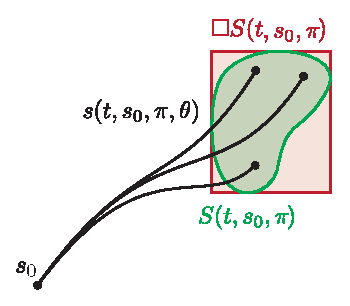
\includegraphics[width=0.5\textwidth]{img/interval-hull}
    \caption{A few trajectories are sampled from an initial state $x_0$ following a policy $\pi=(u_0,\cdots)$ with various parameters $\theta$ (in black). The union of reachability sets is shown in green, and its interval hull in red.}
    \label{fig:interval-hull}
\end{figure}

In order to use the interval predictor from \citep{leurent2019interval}, we also require $A_0$ to be Metzler. This can be ensured under some conditions:

\begin{lemma}[Similarity transformation \citep{Efimov_a2013}]
\label{lem:metzler} Let $D\in\Xi\subset\Real^{n\times n}$ be a matrix variable satisfying the interval constraints $\Xi=\{D\in\Real^{n\times n}:\,D_{a}-\Delta\le D\le D_{a}+\Delta\}$ for some $D_{a}^{\text{T}}=D_{a}\in\Real^{n\times n}$ and $\Delta\in\Real_{+}^{n\times n}$. If for some constant $\mu\in\Real_{+}$ and a diagonal matrix $\Upsilon\in\Real^{n\times n}$ the Metzler matrix $Y=\mu E_{n\times n}-\Upsilon$ has the same eigenvalues as the matrix $D_{a}$, then there is an orthogonal matrix $S\in\Real^{n\times n}$ such that the matrices $S^{\text{T}}DS$ are Metzler for all $D\in\Xi$ provided that $\mu>n||\Delta||_{max}$.\textup{ }
\end{lemma}

\begin{theorem}[Interval Predictor \citep{leurent2019interval}]
\label{thm:predictor}
Assuming that \eqref{eq:polytope} is satisfied for the system \eqref{eq:dynamics}, then the interval predictor:
\begin{eqnarray}
\dot{\underline{x}}(t) & = & A_{0}\underline{x}(t)-\Delta A_{+}\underline{x}^{-}(t)-\Delta A_{-}\overline{x}^{+}(t)\nonumber \\
 &  & +Bu(t)+D^{+}\underline{\omega}(t)-D^{-}\overline{\omega}(t),\nonumber\\
\dot{\overline{x}}(t) & = & A_{0}\overline{x}(t)+\Delta A_{+}\overline{x}^{+}(t)+\Delta A_{-}\underline{x}^{-}(t) \label{eq:interval_predictor} \\
 &  & +Bu(t)+D^{+}\overline{\omega}(t)-D^{-}\underline{\omega}(t),\nonumber \\
 &  & \underline{x}(0)=\underline{x}_{0},\;\overline{x}(0)=\overline{x}_{0}\nonumber 
\end{eqnarray}
ensures the inclusion property \eqref{eq:interval_property}. If there exist diagonal matrices $P$, $Q$, $Q_{+}$, $Q_{-}$, $Z_{+}$, $Z_{-}$, $\Psi_{+}$, $\Psi_{-}$, $\Psi$, $\Gamma\in\Real^{2n\times 2n}$ such that the following LMIs are satisfied:
\begin{gather*}
P+\min\{Z_{+},Z_{-}\}>0,\;\Upsilon\preceq0,\;\Gamma>0,\\
Q+\min\{Q_{+},Q_{-}\}+2\min\{\Psi_{+},\Psi_{-}\}>0,
\end{gather*}
where{\footnotesize{}
\begin{gather*}
\Upsilon=\left[\begin{array}{cccc}
\Upsilon_{11} & \Upsilon_{12} & \Upsilon_{13} & P\\
\Upsilon_{12}^{\top} & \Upsilon_{22} & \Upsilon_{23} & Z_{+}\\
\Upsilon_{13}^{\top} & \Upsilon_{23}^{\top} & \Upsilon_{33} & Z_{-}\\
P & Z_{+} & Z_{-} & -\Gamma
\end{array}\right],\\
\Upsilon_{11}=\mathcal{A}^{\top}P+P\mathcal{A}+Q,\;\Upsilon_{12}=\mathcal{A}^{\top}Z_{+}+PR_{+}+\Psi_{+},\\
\Upsilon_{13}=\mathcal{A}^{\top}Z_{-}+PR_{-}+\Psi_{-},\;\Upsilon_{22}=Z_{+}R_{+}+R_{+}^{\top}Z_{+}+Q_{+},\\
\Upsilon_{23}=Z_{+}R_{-}+R_{+}^{\top}Z_{-}+\Psi,\;\Upsilon_{33}=Z_{-}R_{-}+R_{-}^{\top}Z_{-}+Q_{-},\\
\mathcal{A}=\left[\begin{array}{cc}
A_{0} & 0\\
0 & A_{0}
\end{array}\right],\;R_{+}=\left[\begin{array}{cc}
0 & -\Delta A_{-}\\
0 & \Delta A_{+}
\end{array}\right],\;R_{-}=\left[\begin{array}{cc}
\Delta A_{+} & 0\\
-\Delta A_{-} & 0
\end{array}\right],
\end{gather*}
}then the predictor \eqref{eq:interval_predictor} is input-to-state stable with respect to the inputs $\underline{\omega}$, $\overline{\omega}$.
\end{theorem}

\begin{example*}
Consider a scalar system:
\[
\dot{x}(t)=-\theta(t)x(t)+d(t),\;t\geq0,
\]
where $x(t)\in\Real$ with $x(0)\in[\underline{x}_{0},\overline{x}_{0}]=[1.0, 1.1]$, $\theta(t)\in\Pi=[\underline{\theta},\overline{\theta}]=[0.5,1.5]$ and $d(t)\in[\underline{d},\overline{d}]=[-0.1,0.1]$ for all $t\geq0$. The \autoref{fig:predictor_example} shows the state-interval obtained with \eqref{eq:interval_predictor}.

\begin{figure}
\begin{centering}
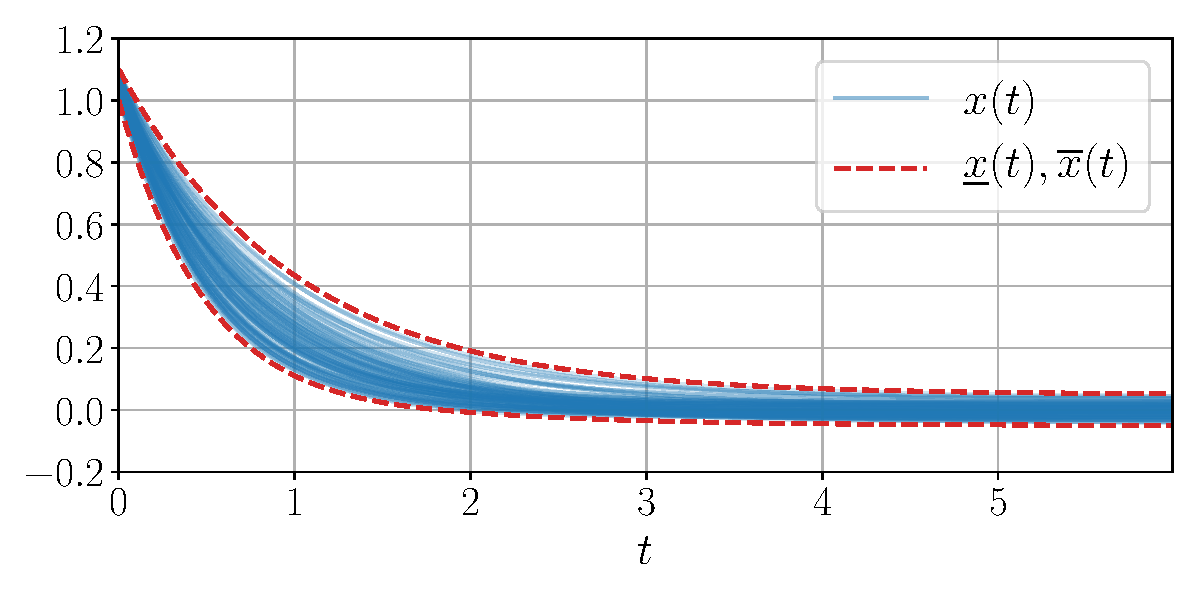
\includegraphics[width=\linewidth]{img/interval_predictor}
\par\end{centering}
\caption{Several trajectories for different values of $\theta\in\Theta$ are shown in blue. The result of prediction by \eqref{eq:interval_predictor} is in red: the predictor is stable and produces tight bounds.}
\label{fig:predictor_example}
\end{figure}
\end{example*}

\section{Control}

In this section, we still assume that we have a high-confidence polytope $\cP$ that verifies \eqref{eq:polytope} with probability $1-\delta$.


The \textbf{robust control} objective $v^r$:
\todo[inline]{EL: since the interval dynamics will be deterministic, use open-loop policies, ie sequences of actions $\mathbf{u}$ instead of closed-loop policies $\pi$}

\begin{equation}
\label{eq:robust-control}
\max_\pi \underbrace{\min_{\theta \in \Theta} \expectedvalueover{\omega(t)}\left[\sum_{t=0}^\infty \gamma^t r(x(t))\condbar \dot{x}(t) = A(\theta) x(t) + B_u u(t) + B_\omega\omega(t), u_t = \pi(x_t)\right]}_{v^r(\pi)}
\end{equation}


\begin{definition}[Surrogate objective]
We modify the robust objective $v^r$ in \eqref{eq:robust-control} by replacing the true reachability set by its interval prediction $[\underline{x}(t), \overline{x}(t)]$ based on the polytopic approximation $\cP_\delta$ of $A(\Theta)$: 

\begin{equation}
\hat{v^r}(\pi) \eqdef \sum_{t=0}^\infty \gamma^t \min_{x\in[\underline{x}(t, \pi), \overline{x}(t, \pi)]}  r(x)
\end{equation}
where $\underline{x}(t, \pi), \overline{x}(t, \pi)$ follow the dynamics defined in \eqref{eq:interval_predictor}.
\end{definition}

\begin{algorithm}[tp]
  \SetAlgoLined\DontPrintSemicolon
  \SetKwFunction{algo}{robust\_control}
  \SetKwFunction{proc}{pessimistic\_reward}
  \SetKwProg{myalg}{Algorithm}{}{}
  \myalg{\algo{$s_0$}}{
  \While{resources available}
  {
  Generate a candidate sequence $\pi$ with a planning algorithm using \proc{} instead of the true rewards.
  }
  \KwRet $\argmax_{\pi\in\Pi} \hat{v^r}(\pi)$ \;}{}
  \setcounter{AlgoLine}{0}
  \SetKwProg{myproc}{Procedure}{}{}
  \myproc{\proc{$s_0$, $\pi$, T}}{
  Integrate \eqref{eq:interval_predictor} over $[0,t]$ with commands $\pi$ to compute $[\underline{x}(t), \overline{x}(t)]$\;
  \KwRet $\min_{x\in[\underline{x}(t), \overline{x}(t)]} r(x)$\;}
\caption{Interval-based Robust Control}
\label{algo:irc}

\end{algorithm}

\begin{property}[Lower bound]
\label{prop:lower-bound}
With high probability, the surrogate objective $\hat{v^r}$ is a lower bound of the true objective $v^r$:

\begin{equation}
\probability{\forall \pi, \hat{v^r}(\pi) \leq v^r(\pi)} \geq 1-\delta
\end{equation}
\end{property}

\begin{proof}
Let $\theta\in\Theta$, by \autoref{thm:confidence_interval} we have that $A(\theta) \in \cP$ with probability $1-\delta$. Whenever it is the case, we have by \autoref{thm:predictor} that the inclusion property \eqref{eq:interval_property} is verified by the interval predictor \eqref{eq:interval_predictor} for all $\omega(t)\in[\underline{\omega}(t), \overline{\omega}(t)]$. This gives the following bound:
\begin{equation*}
 \sum_{t=0}^\infty \gamma^t r(x_t) \geq \sum_{t=0}^\infty \min_{x\in[\underline{x}(t, \pi), \overline{x}(t, \pi)]} \gamma^t r(x) = \hat{v^r}(\pi)
\end{equation*}

And finally, with probability $1-\delta$,
\begin{align*}
v^r(\pi) &= \min_{A(\theta) \in A(\Theta)} \expectedvalueover{\omega(t)}\left[\sum_{t=0}^\infty \gamma^t r(x_t)\right] \\
&\geq \min_{A \in \cP} \expectedvalueover{\omega(t)}\left[\sum_{t=0}^\infty \gamma^t r(x_t)\right] \\
& \geq \min_{A \in \cP} \expectedvalueover{\omega(t)}\left[\hat{v^r}(\pi)\right] = \hat{v^r}(\pi)
\end{align*}
\end{proof}

The robust objective error $v^r - \hat{v^r}$ stems from two terms: the approximation of the reachable set by the polytopic and interval approximations and the loss of time-dependency between the states within a single trajectory. If both these approximations are tight enough, maximizing the lower bound $\hat{v^r}$ will increase the true objective $v^r$, which is the idea behind Algorithm \ref{algo:irc}.

\section{Multi-model Estimation and Control}

\subsection{Model adequacy}
\subsection{Robust control with Discrete Ambiguity}


\begin{assumption}[Multi-model ambiguity]
Assume that the true dynamics $f$ lies within a finite set of candidate models $f^1, \cdots, f^M$.
\begin{equation}
\exists m\in[M]: \dot{x}(t) = f^M(x(t), u(t)), \forall t\geq 0
\end{equation}

We temporarily ignore the parametric uncertainty $\theta\in\Theta$ to only consider known deterministic models.
\end{assumption}

\begin{definition}[Robust sequence upper bounds] We define an upper-bound for the value of sequences of actions:
\begin{equation}
\label{eq:robust_sequence_ucb}
b_i^r(n)  \eqdef
\begin{cases}
\min_{m\in[1, M]} \sum_{t=0}^{d-1} \gamma^t r_t^m  + \frac{\gamma^d}{1-\gamma} &\text{if } i \in \mathcal{L}_n \text{ ;}\\
\max_{a\in\mathcal{A}} b_{ia}^r(n) & \text{if } i \in \mathcal{T}_n \setminus \mathcal{L}_n 
\end{cases}
\end{equation}
where $r_t^m$ is the reward obtained at step $t$ by following $i$ with dynamics $f^m$.
\end{definition}
An illustration of the computation of the robust b-values is presented in Figure \ref{fig:drop}.


\begin{figure}
\centering
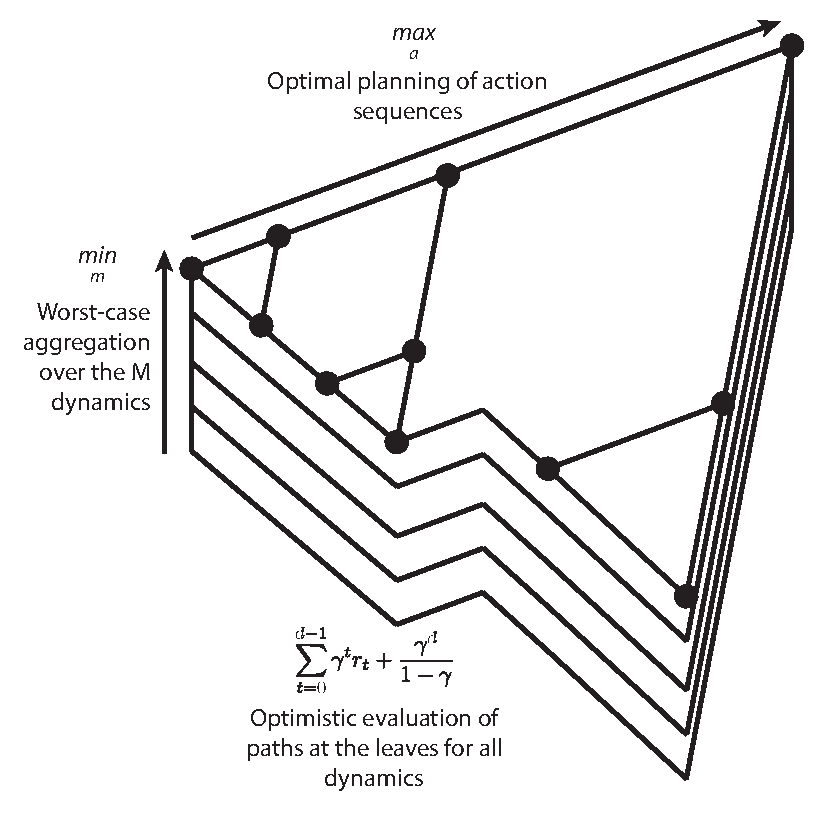
\includegraphics[width=0.5\linewidth]{img/robust-control-tree}
\caption{The computation of robust b-values in Algorithm \ref{algo:drop}. The simulation of trajectories for every dynamics model $f^m$ is represented as stacked versions of the expanded tree $\mathcal{T}_n$.}
\label{fig:drop}
\end{figure}

From this definition we introduce Algorithm \ref{algo:drop}, and analyse its sample-efficiency in Theorem \ref{theorem:drop-regret}.

\begin{algorithm}[tp]
\DontPrintSemicolon
Initialize $\mathcal{T}$ to a root and expand it. Set $n=1$.\;
\While{Numerical resource available}{
Compute the robust u-values $u^r_i(n)$ and robust b-values $b^r_i(n)$.\;
Expand $\argmax_{i\in \mathcal{L}_n} b^r_i(n)$.\;
n = n + 1\;
}
\Return $\argmax_{a\in \mathcal{A}} u^r_a(n)$
\caption{Deterministic Robust Optimistic Planning}
\label{algo:drop}
\end{algorithm}

The simple regret of the action $a$ returned by Algorithm \ref{algo:drop} after $n$ rounds is defined as:
\begin{equation}
\mathcal{R}_n = v^r - v_a^r
\end{equation}
We will say that $\mathcal{R}_n=O(\varepsilon)$ for some $\varepsilon>0$ if there exist $\rho>0$ and $n_0>0$ such that $\mathcal{R}_n\leq\rho\varepsilon$ for all $n\geq n_0$.
A node $i\in\mathcal{T}$ is said to be $\epsilon$-optimal, in a robust sense, if and only if $v_i^r \geq v^r - \epsilon$ for some $\epsilon > 0$. The proportion of $\epsilon$-optimal nodes at depth $d$ is then defined as $p_d(\epsilon) = |i \in \mathcal{A}^d$ s.t $i$ is $\epsilon$-optimal$|/K^d$. Further we will assume that for the graph $\mathcal{T}$ the following hypothesis is satisfied:
\begin{assumption}[Proportion of near-optimal nodes]
\label{assumpt:beta}
There exist $\beta\in[0, \frac{\log K}{\log 1/\gamma}]$, $c > 0$ and $d_0 > 0$ such that $p_d(\epsilon)\leq c\epsilon^\beta$ for all $\epsilon > 0$ and $d\geq d_0$.
\end{assumption}

\begin{theorem}[Regret bound]
\label{theorem:drop-regret}
Let $\kappa = K\gamma^\beta \in [1, K]$. Then the simple regret of Algorithm \ref{algo:drop} is:


\begin{equation}
\text{If } \kappa>1,\qquad 
\mathcal{R}_n = O\left(n^{-\frac{\log 1/\gamma}{\log \kappa}}\right)
\end{equation}

\begin{equation}
\text{If }\kappa=1,\qquad
\mathcal{R}_n = O\left(\gamma^{\frac{(1-\gamma)^\beta}{c}n}\right)
\end{equation}
\end{theorem}

\section{The Use-Case of Autonomous Driving}


We consider the problem of safe decision-making for autonomous highway driving. An autonomous vehicle is driving on a highway populated with $N$ other agents, and uses Model Predictive Control to plan a sequence of decisions. To that end, it relies on parametrized dynamical model for each agent to predict the future trajectory of each traffic participant: \[\dot{z}_i=f_i(Z,\theta_i),\;i=\overline{1,N},\] where $f_i$ are described below, $z_i\in\Real^4$ is the state of an agent, $Z = [z_1,\dots,z_N]^\top\in\Real^{4N}$ and $\theta_i\in\Real^5$ is the corresponding vector of unknown parameters. Crucially, this system describes the couplings and interactions between vehicles, so that the autonomous agent can properly anticipate their reactions. 
However, we assume that we do not have access to the true values of the behavioural parameters $\theta=[\theta_1,\dots,\theta_N]^\top$; instead, we merely know that these parameters lie in a set of admissible values $\Pi\subset\Real^{5N}$. In order to act safely in the face of uncertainty, we follow the framework of robust decision-making: the agent must consider all the possible trajectories in the space of $Z$ that each vehicle can follow in order to take its decisions. In this work, we focus on how to compute these trajectory enclosures through interval prediction.

In the following, we describe the system and its associated interval predictor.

\subsection{Kinematics}

The kinematics of any vehicle $i\in\overline{1,V}$ are represented by the Kinematic Bicycle Model:
\begin{align}
	\dot{x}_i &= v_i\cos(\psi_i), \nonumber\\
	\dot{y}_i &= v_i\sin(\psi_i), \nonumber\\
	\dot{v}_i &= a_i, \nonumber\\
	\dot{\psi}_i &= \frac{v_i}{l}tan(\beta_i), \nonumber
\end{align}
where $(x_i, y_i)$ is the vehicle position, $v_i$ is its forward velocity and $\psi_i$ is its heading, $l$ is the vehicle half-length, $a_i$ is the acceleration command and $\beta_i$ is the slip angle at the centre of gravity, used as a steering command.

\subsection{Longitudinal control}
Longitudinal behaviour is modelled by a linear controller using three features inspired from the intelligent driver model (IDM) \cite{Treiber2000}: a desired velocity, a braking term to drive slower than the front vehicle, and a braking term to respect a safe distance to the front vehicle.

Denoting $f_i$ the index of the front vehicle preceding vehicle $i$, the acceleration command can be presented as follows:
\begin{equation*}
	a_i = \begin{bmatrix}
	\theta_{i,1} & \theta_{i,2} & \theta_{i,3}
	\end{bmatrix} \begin{bmatrix}
		v_0 - v_i \\
		-(v_{f_i}-v_i)^- \\
		-(x_{f_i} - x_i - (d_0 + v_iT))^- \\
	\end{bmatrix},
	\label{eq:theta_a}
\end{equation*}
where $v_0, d_0$ and $T$ respectively denote the speed limit, jam distance and time gap given by traffic rules.

\subsection{Lateral control}

The lane $L_i$ with the lateral position $y_{L_i}$ and heading $\psi_{L_i}$ is tracked by a cascade controller of lateral position and heading $\beta_i$, which is selected in a way the closed-loop dynamics take the form:

\begin{align}
	\label{eq:heading-command}
    \dot{\psi}_i &= \theta_{i,5}\left(\psi_{L_i}+\sin^{-1}\left(\frac{\tilde{v}_{i,y}}{v_i}\right)-\psi_i\right),\\
    \tilde{v}_{i,y} &= \theta_{i,4} (y_{L_i}-y_i). \nonumber
\end{align}
We assume that the drivers choose their steering command $\beta_i$ such that \eqref{eq:heading-command} is always achieved: $\beta_i = \tan^{-1}(\frac{l}{v_i}\dot{\psi}_i)$.

\subsection{LPV formulation}

The system presented so far is non-linear and must be cast into the LPV form. We approximate the non-linearities induced by the trigonometric operators through equilibrium linearisation around $y_i=y_{L_i}$ and $\psi_i=\psi_{L_i}$.

This yields the following longitudinal dynamics:
\begin{align*}
\dot{x}_i &= v_i,\\
\dot v_i &= \theta_{i,1} (v_0 - v_i) + \theta_{i,2} (v_{f_i} - v_i) + \theta_{i,3}(x_{f_i} - x_i - d_0 - v_i T),
\end{align*}
where $\theta_{i,2}$ and $\theta_{i,3}$ are set to $0$ whenever the corresponding features are not active.

It can be rewritten in the form $$\dot{Z} = A(\theta)(Z-Z_c) + d.$$ For example, in the case of two vehicles only:
\begin{equation*}
    Z = \begin{bmatrix}
x_i \\
x_{f_i} \\
v_i \\
v_{f_i} \\
\end{bmatrix}
,\quad
Z_c = \begin{bmatrix}
-d_0-v_0 T \\
0 \\
v_0\\
v_0 \\
\end{bmatrix}
,\quad
d = \begin{bmatrix}
v_0 \\
v_0 \\
0\\
0\\
\end{bmatrix}
\end{equation*}

\begin{equation*}
A(\theta)
=
\begin{blockarray}{ccccc}
 & i & f_i & i & f_i \\
\begin{block}{c[cccc]}
i & 0 & 0 & 1 & 0 \\
f_i & 0 & 0 & 0 & 1 \\
i & -\theta_{i,3} & \theta_{i,3} & -\theta_{i,1}-\theta_{i,2}-\theta_{i,3} & \theta_{i,2} \\
f_i & 0 & 0 & 0 & -\theta_{f_i,1} \\
\end{block}
\end{blockarray}
\end{equation*}

The lateral dynamics are in a similar form:
\begin{equation*}
\begin{bmatrix}
\dot{y}_i \\
\dot{\psi}_i \\
\end{bmatrix}
=
\begin{bmatrix}
0 & v_i \\
-\frac{\theta_{i,4} \theta_{i,5}}{v_i} & -\theta_{i,5}
\end{bmatrix}
\begin{bmatrix}
y_i - y_{L_i} \\
\psi_i - \psi_{L_i}
\end{bmatrix}
+
\begin{bmatrix}
v_i\psi_{L_i} \\
0
\end{bmatrix}
\end{equation*}
Here, the dependency in $v_i$ is seen as an uncertain parametric dependency, \emph{i.e.} $\theta_{i,6}=v_i$, with constant bounds assumed for $v_i$ using an overset of the longitudinal interval predictor.

\subsection{Change of coordinates}
In both cases, the obtained polytope centre $A_0$ is non-Metzler.
We use lemma \ref{lem:metzler} to compute a similarity transformation of coordinates. Precisely, we ensure that the polytope is chosen so that its centre $A_0$ is diagonalisable having real eigenvalues, and perform an eigendecomposition to compute its change of basis matrix $S$. The transformed system $Z'=S^{-1}(Z-Z_c)$ verifies \eqref{eq:polytope} with $A_0$ Metlzer as required to apply the interval predictor of Theorem~\ref{thm:predictor}. Finally, the obtained predictor is transformed back to the original coordinates $Z$ by using the interval arithmetic of Lemma~\ref{lem:interval}.


\printbibliography

\end{document}
